% Document : compte rendu des DM
% Auteur : Xavier Gandibleux
% Année académique : 2018-2019

\documentclass[a4paper,10pt]{article}


% passe en mode large sur la page A4
\usepackage{a4wide} 

% document francisé
\usepackage[francais]{babel} 

% permet la frappe de caracteres accentues (sur macOS)
\usepackage[utf8x]{inputenc} 

\usepackage{graphicx,float,subcaption} % figure et placement de figure
\usepackage[top=10mm, bottom=10mm, left=15mm, right=10mm]{geometry}

\usepackage{multicol}
%\usepackage[T1]{fontenc}
%\usepackage{graphicx}
%\usepackage{grffile}
%\usepackage{longtable}
%\usepackage{wrapfig}
%\usepackage{rotating}
%\usepackage[normalem]{ulem}
%\usepackage{amsmath}
%\usepackage{textcomp}
%\usepackage{amssymb}
%\usepackage{capt-of}
%\usepackage{hyperref}% \documentclass[a4paper,11pt]{article}
% \usepackage[margin=2cm]{geometry}
% \usepackage[utf8]{inputenc}

%\usepackage{graphicx} 
%\usepackage{wrapfig}
\usepackage{color}
\usepackage{xcolor}
%\usepackage{hyperref}


%\usepackage[]{amsmath,amsfonts,amssymb,stmaryrd,amsthm}
%\usepackage{fullpage}
%\usepackage{multirow}
%\usepackage[rounded]{syntax}
%\usepackage[section]{placeins}
\newtheorem{example}{Exemple} %%% modifier ici si on veut en fr/en

\usepackage{todonotes}
\usepackage{listings} 


\usepackage{listings}
\usepackage{inconsolata} % very nice fixed-width font included with texlive-full
%\usepackage[usenames,dvipsnames]{color} % more flexible names for syntax highlighting colors

\definecolor{chameleond}{HTML}{4E9A06}
\definecolor{skyblued}{HTML}{204A87}
\definecolor{darkgreen}{HTML}{006400}

%\usepackage[usenames,dvipsnames]{color} % more flexible names for syntax highlighting colors


\lstset{
basicstyle=\ttfamily, 
columns=fullflexible, % make sure to use fixed-width font, CM typewriter is NOT fixed width
numbers=left, 
numberstyle=\small\ttfamily\color{gray},
stepnumber=1,              
numbersep=10pt, 
numberfirstline=true, 
numberblanklines=true, 
tabsize=4,
lineskip=-1.5pt,
extendedchars=true,
breaklines=true,        
keywordstyle=\color{skyblued}\bfseries,
identifierstyle=, % using emph or index keywords
commentstyle=\sffamily\color{darkgreen},
stringstyle=\color{chameleond},
showstringspaces=false,
showtabs=false,
upquote=false,
texcl=true % interpet comments as LaTeX
}


\lstset{literate=
  {α}{{$\alpha$}}1 {Δ}{{$\Delta$}}1
  {á}{{\'a}}1 {é}{{\'e}}1 {í}{{\'i}}1 {ó}{{\'o}}1 {ú}{{\'u}}1
  {Á}{{\'A}}1 {É}{{\'E}}1 {Í}{{\'I}}1 {Ó}{{\'O}}1 {Ú}{{\'U}}1
  {à}{{\`a}}1 {è}{{\`e}}1 {ì}{{\`i}}1 {ò}{{\`o}}1 {ù}{{\`u}}1
  {À}{{\`A}}1 {È}{{\'E}}1 {Ì}{{\`I}}1 {Ò}{{\`O}}1 {Ù}{{\`U}}1
  {ä}{{\"a}}1 {ë}{{\"e}}1 {ï}{{\"i}}1 {ö}{{\"o}}1 {ü}{{\"u}}1
  {Ä}{{\"A}}1 {Ë}{{\"E}}1 {Ï}{{\"I}}1 {Ö}{{\"O}}1 {Ü}{{\"U}}1
  {â}{{\^a}}1 {ê}{{\^e}}1 {î}{{\^i}}1 {ô}{{\^o}}1 {û}{{\^u}}1
  {Â}{{\^A}}1 {Ê}{{\^E}}1 {Î}{{\^I}}1 {Ô}{{\^O}}1 {Û}{{\^U}}1
  {œ}{{\oe}}1 {Œ}{{\OE}}1 {æ}{{\ae}}1 {Æ}{{\AE}}1 {ß}{{\ss}}1
  {ű}{{\H{u}}}1 {Ű}{{\H{U}}}1 {ő}{{\H{o}}}1 {Ő}{{\H{O}}}1
  {ç}{{\c c}}1 {Ç}{{\c C}}1 {ø}{{\o}}1 {å}{{\r a}}1 {Å}{{\r A}}1
  {€}{{\EUR}}1 {£}{{\pounds}}1
}

% \lstset{language=bash,
% stringstyle=\ttfamily,
% basicstyle=\footnotesize, 
% showstringspaces=false,
% breaklines=true,
% }

\lstdefinestyle{numbers} {numbers=left, stepnumber=5, numberstyle=\tiny, numbersep=10pt}
% \lstdefinestyle{lc3} {language=[x86masm]Assembler,style=numbers,frame=lines,showstringspaces=false,keywords={BR,LD,BRz,BRn,BRzp,BRnz,BRnzp,LEA,HALT,RET,.END,.ORIG,.FILL,.STRINGZ,PUTS,ADD,AND,OR,OUT,NOT,LDR,STR,JSR,NOP,GETC},showstringspaces=false,keepspaces=true,flexiblecolumns=true,deletekeywords={end}}

\lstdefinestyle{target}
{language=[x86masm]Assembler,style=numbers,frame=lines,showstringspaces=false,keywords={add,
  jump, snif,call,return,.string,.reserve,.word,.set,.align16,letl,leth,.let,and,or,wmem,rmem,asr,xor,sub,sgt,sle,slt,slt},showstringspaces=false,keepspaces=true,flexiblecolumns=true,deletekeywords={end},breaklines=true}



%\definecolor{chameleond}{HTML}{4E9A06}
%\definecolor{skyblued}{HTML}{204A87}


\lstdefinestyle{digmips} {language=[x86masm]Assembler,style=numbers,frame=lines,showstringspaces=false,keywords={add,sub,ld,ldi,ble,j,jmp,st},showstringspaces=false,keepspaces=true,flexiblecolumns=true,deletekeywords={end},keywordstyle=\color{skyblued},commentstyle=\color{red}\bf,morecomment=[l][\color{red}]{//}}


\lstdefinestyle{lc3} {language=[x86masm]Assembler,style=numbers,frame=lines,showstringspaces=false,keywords={BR,LD,BRz,BRn,BRzp,BRnz,BRnzp,LEA,HALT,RET,.END,.ORIG,.FILL,.STRINGZ,PUTS,ADD,AND,OR,OUT,NOT,LDR,STR,JSR,NOP,GETC},showstringspaces=false,keepspaces=true,flexiblecolumns=true,deletekeywords={end}}


\lstdefinelanguage{[Objective]Caml}
{basicstyle=\ttfamily,
keywordstyle=\itshape\bfseries,
identifierstyle=,
stringstyle=\itshape,
commentstyle=\itshape,
flexiblecolumns=true,
escapechar=\%}

\lstdefinelanguage{julia}
{
  keywordsprefix=\@,
  morekeywords={
    exit,whos,edit,load,is,isa,isequal,typeof,tuple,ntuple,uid,hash,finalizer,convert,promote,
    subtype,typemin,typemax,realmin,realmax,sizeof,eps,promote_type,method_exists,applicable,
    invoke,dlopen,dlsym,system,error,throw,assert,new,Inf,Nan,pi,im,begin,while,for,in,return,
    break,continue,macro,quote,let,if,elseif,else,try,catch,end,bitstype,ccall,do,using,module,
    import,export,importall,baremodule,immutable,local,global,const,Bool,Int,Int8,Int16,Int32,
    Int64,Uint,Uint8,Uint16,Uint32,Uint64,Float32,Float64,Complex64,Complex128,Any,Nothing,None,
    function,type,typealias,abstract
  },
  sensitive=true,
  morecomment=[l]{\#},
%  morecomment=[s]{# =}{=#},
  morestring=[b]',
  morestring=[b]" 
}

\lstdefinelanguage{cplus}
{
        frame=lines,
	language=C++,
	basicstyle=\tt,
        morecomment=[l][\color{magenta}]{\#},
	keywordstyle=\color{chameleond},
	identifierstyle=\color{black},
        stringstyle=\color{skyblued},
        commentstyle=\color{red},
	tabsize=4,
}


\lstdefinelanguage{mypython}
{
%        frame=lines,
	language=Python,
	basicstyle=\tt,
        morecomment=[l][\color{magenta}]{\#},
	keywordstyle=\color{chameleond},
	identifierstyle=\color{black},
        stringstyle=\color{skyblued},
        commentstyle=\color{red},
	tabsize=4,
        breaklines=true,
}


\lstdefinelanguage{flexbison}
{
        frame=lines,
	language=C,
	basicstyle=\tt,
        keywords={yylex,yyparse,yyline,yytext,yyin},
        morecomment=[l][\color{magenta}]{\#,},
	keywordstyle=\color{chameleond},
	identifierstyle=\color{black},
        stringstyle=\color{skyblued},
        commentstyle=\color{red},
	tabsize=4,
}


\lstdefinelanguage{antlr}
{
%  frame=lines,
  language=Java,
  basicstyle=\tt\scriptsize,
  breaklines=true,%                                      allow line breaks
  moredelim=[s][\color{blue!50!black}\ttfamily]{'}{'},% single quotes in green
  moredelim=*[s][\color{black}\ttfamily]{options}{\}},%  options in black (until trailing })
  commentstyle={\color{gray}\itshape},%                  gray italics for comments
  morecomment=[l]{//},%                                  define // comment
  emph={%
    STRING%                                            literal strings listed here
  },emphstyle={\color{blue}\ttfamily},%              and formatted in
                                %              blue
  keywords={grammar,header,members,skip},
  alsoletter={:,|,;},%
  morekeywords={:,|,;},%                                 define the special characters
  keywordstyle={\color{chameleond}},%                         and format them in black
}


\lstdefinelanguage{mycaml}
{       language=Caml,
        upquote=true,
        columns=flexible,
        keepspaces=true,
        breakindent=0pt,
        basicstyle=\ttfamily,
        breaklines=true,
        keywordstyle=\color{red},
        commentstyle=\color{darkgreen},
        tabsize=2,
        escapechar=\%,
        escapebegin=\color{blue}
        }

\lstdefinelanguage{myhaskell}
{       language=Haskell,
        upquote=true,
        columns=flexible,
        keepspaces=true,
        breakindent=0pt,
        basicstyle=\ttfamily\scriptsize,
        breaklines=true,
        keywordstyle=\color{red},
        commentstyle=\color{darkgreen},
        tabsize=2,
        escapeinside={!}{!},
        escapebegin=!\endgraf\color{gray},
        }



\newcommand\ocamli[1]{\lstinline[language=mycaml,basicstyle=\ttfamily\normalsize]{#1}}
\newcommand\llvminline[1]{\lstinline[language=LLVM,basicstyle=\ttfamily\normalsize]{#1}}
\newcommand\llvmfile[1]{\lstinputlisting[language=LLVM]{#1}}

\lstnewenvironment{llvmc}{
  \lstset{language=llvm,mathescape,
    basicstyle=\ttfamily\small,
    aboveskip={0\baselineskip},
    belowskip=0\baselineskip
  }}{}


\lstdefinelanguage{lustre}
{
  basewidth={0.5em,0.5em},
  % list of keywords
  morekeywords={
    pre,
    fby,
    ->,
    current,
    when,
    node, 
    returns,
    let,
    tel,
    var,
    if,
    then,
    int,
    bool,
  },
  sensitive=false, % keywords are not case-sensitive
  escapeinside={!}{!},          % if you want to add LaTeX within your code
  morecomment=[l]{//}, % l is for line comment
  morecomment=[s]{/*}{*/}, % s is for start and end delimiter
  morestring=[b]", % defines that strings are enclosed in double quotes
  basicstyle=\ttfamily,
  keywordstyle=\bfseries\color{blue!80!black},
  keywordstyle=[2]\bfseries\color{red!50!white},
  commentstyle=\itshape\color{purple!40!black},
  %identifierstyle=\color{blue!80!black},
  stringstyle=\color{orange}
}


\newcommand{\arthur}[1]{\textcolor{violet}{#1}}
\newcommand{\marie}[1]{\textcolor{red}{#1}}
\newcommand{\prof}[1]{\textcolor{gray}{#1}}

%% IL faut mettre le package pour tabular 


% individualisation des parametres de la page
\parskip8pt
\setlength{\topmargin}{-25mm}
\setlength{\textheight}{250mm}

%
% -----------------------------------------------------------------------------------------------------------------------------------------------------
%

\begin{document}
\pagestyle{empty}
{\begin{center}
  {  \fbox{Langages de programmation de haut niveau}\\
      \vspace{1mm}
  \begin{minipage}{0.45 \textwidth}
	\begin{flushleft}
     Rapport TP1 R
	\end{flushleft}
  \end{minipage}
  \begin{minipage}{0.45 \textwidth}
	\begin{flushright}
     Marie Humbert--Ropers ; Arthur Gontier
	\end{flushright}
  \end{minipage}
  }  
\end{center}
}
      %\vspace{1mm}
%\noindent
\fbox{
  \begin{minipage}{0.97 \textwidth}
    \begin{center}
      \vspace{1mm}
	{a) Comparaisons des temps de calculs}
      \vspace{1mm}
    \end{center}
  \end{minipage}
}
\vspace{1mm}
\begin{multicols}{2}
	\par{
Sur 1 000 000 d'itérations, on obtient les temps de calculs suivants :\\
    \begin{tabular}{|c|c|c|c|}
    \hline
     fonction & utilisateur & système & écoulé\\
     \hline
     rectangle & 0.546 & 0.00 & 0.545\\
     \hline
     rectangle1l & 0.119 & 0.004 & 0.123\\
     \hline
     montecarlo & 3.968 & 0.004 & 3.971\\
     \hline
     montecarlo1l & 0.107 & 0.004 & 0.110\\
     \hline
    \end{tabular}
}
\par{
Pour chaque méthode, il existe deux versions: l'une utilisant les fonctions des bibliothèques de R et l'autre n'utilisant que des boucles.\\
	Nous pouvons donc remarquer que les fonctions utilisant le plus possible les bibliothèques compilés de R sont 5 fois plus rapides pour la méthode du rectangle, et 40 fois plus rapides pour la méthode de Monte-Carlo.
}
\end{multicols}
Pour la suite, nous utilisons uniquement les versions rapides de ces algorithmes.

\vspace{1mm}
\noindent
\fbox{
  \begin{minipage}{0.97 \textwidth}
    \begin{center}
      \vspace{1mm}
      {b) Précision du résultat en fonction de n}
      \vspace{1mm}
    \end{center}
  \end{minipage}
}
%\vspace{1mm}

On note que l'on compare ici les résultats avec la valeur "exacte" donnée par la machine, qui n'est pas complètement exact mais, en admettant qu'elle en est très proche, cela donne un ordre d'idée concernant la précision de ces méthodes. \\
%Pour cette même raison, nous présentons un graphe avec la droite "exacte" et les autres résultats.\\
\begin{minipage}{0.5\textwidth}
\begin{flushleft}
      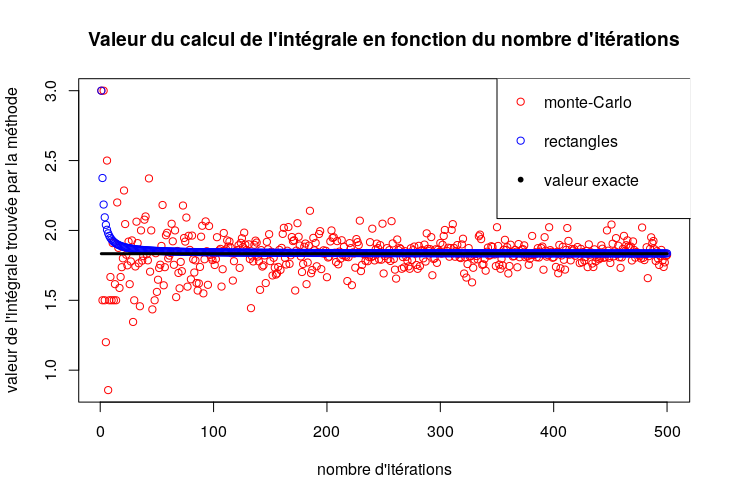
\includegraphics[scale=0.5]{fig/precision_iteration.png}
\end{flushleft}
\end{minipage}
\hspace{1cm}
\begin{minipage}{0.45\textwidth}
	Nous remarquons que la méthode des rectangles converge très rapidement, au bout d'une cinquantaine d'itérations vers la solution exacte avec une précision de l'ordre du millième. La méthode aléatoire de monte-carlo finit aussi par converger mais avec une plus grande lenteur et une moins grande précision. L'exemple ci-contre a été réalisé avec 500 itérations, nous avons aussi constaté que la convergence s'accentue pour un plus grand nombre d'itérations. La précision dans cet exemple varie de 0.005 pour la méthode des rectangles contrairement à 0.1 dans le pire des cas pour la méthode de monte-carlo. On remarque via le vecteur des résultats que la précision de cette dernière est moins constante sur les résultats que celle avec les rectangles: la précision peut-être très bonne puis très mauvaise à l'itération suivante.
\end{minipage}

\vspace{1mm}
\noindent
\fbox{
  \begin{minipage}{0.97 \textwidth}
    \begin{center}
      \vspace{1mm}
      {c) précision du résultat en fonction du temps de calcul}
      \vspace{1mm}
    \end{center}
  \end{minipage}
}
\vspace{1mm}

Dans cette partie, nous avons mesuré pour chaque pas de temps (ici 0.009s), quel était le résultat de chaque méthode
\begin{minipage}{0.5\textwidth}
\begin{flushleft}
      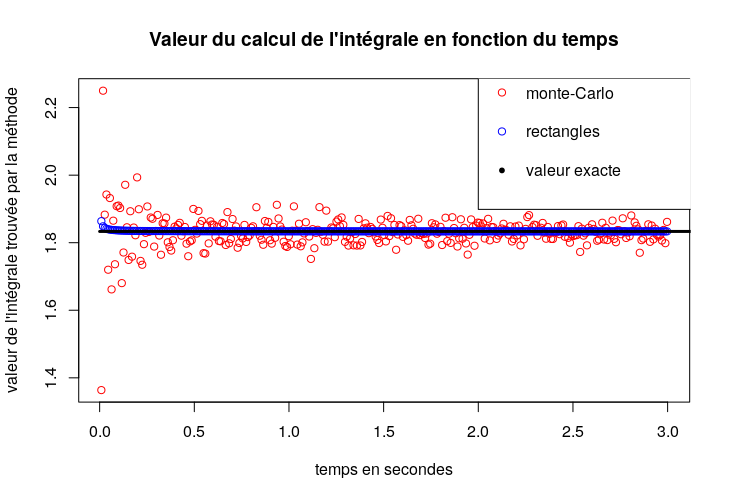
\includegraphics[scale=0.5]{fig/precision_temps.png}
\end{flushleft}
\end{minipage}
\hspace{1cm}
\begin{minipage}{0.45\textwidth}
	Comme précèdemment, nous remarquons que sur 3 secondes d'itérations, la convergence de la méthode des rectangles est très rapide: autour de 0.2 secondes. Pour la méthode aléatoire de monte-carlo, nous constatons que la méthode à tendance à se rapprocher de la valeur "exacte" retenue par la machine. Par calcul, nous vérifions que la précision varie toujours de plus/moins 0.0001 pour la méthode des rectangles contrairement à celle de monte-carlo dont la précision varie de 0.05.


\end{minipage}


\end{document}

